\documentclass[notitlepage]{article}

\usepackage{amssymb}
\usepackage{amsmath}
\usepackage{graphicx}
\usepackage{dcolumn}
\usepackage{hyperref}
\usepackage{algpseudocode,caption}
\usepackage{listings}
\usepackage{color}

\DeclareCaptionType{algorithm}

\begin{document}
\lstset{language=matlab}

\title{Reactive Programming Tutorial in Javascript for Engineers}
\author{Rodrigo Setti \texttt{rodrigosetti@gmail.com}}

\maketitle

\begin{abstract}
    This tutorial makes use of a simple Javascript library to demonstrate some
    working examples of the reactive programming paradigm. It's a way of
    programming where one specifies what is the data flow architecture, instead
    of defining how the data should be processed. Spreadsheets are one notable
    example of a successful application of this paradigm, but I argue that it
    can be extended to general programming, not to solve all kinds of problems
    of course, but it is a nice abstraction to have in the software engineer
    toolbox.
\end{abstract}

\section{Introduction}

Reactive Programming is a programming paradigm where the programmer specifies
declaratively what is the data flow path, instead of specifying how the
processing responds to data changes.

More concretely, and as an example in a finance application, instead of
specifying that ``once the user enter new expenses, the total should be
updated'', in the reactive paradigm one just encodes that ``the total is the
sum of expenses'', and the framework takes care of the ``flow'' and ``event
handling'', \textit{i.e.} reacting to changes in data.

This way of programming is very convenient in may domains, notably in user
input driven applications, as well as simulations that involve processing of
values that varies in time.

Spreadsheets (like Microsoft Excel) let you declare values that depend on other
values (using formulas), and they ``react'' to changes automatically by
updating themselves. Thus, not requiring the user to program the details of
event handling and propagation of changes in complex chain reactions of values
changes.

This tutorial uses a very simple library for reactive programming written in
Javascript. Why Javascript? Well, it's a widely used language, so I hope that
fact contributes to this text being accessible to more programmers.

The library is written in under 150 lines of code \- and it's able to achieve a
lot. This library (called \texttt{rp}, and available at
\texttt{https://github.com/rodrigosetti/rpjs}) is specialized in time-based
reactive values (\textit{i.e.} values that varies in time), but reactive
programming is something much more general and can be used to model any sort of
reactive value (not just ones that varies in time).

\texttt{rp} has two concepts that we are going to talk about:

\begin{itemize}
    \item \textit{Signals}: which are values (any kind of value) that varies in
        time. You can think of a signal being a function from time to value.
    \item \textit{Signal Functions}: which are transformations from one signal
        to another. Signal functions are the main abstraction building blocks
        that we are going to use. In fact, as a user of the library, you can't
        just go ahead and create a signal, all is constructed in terms of
        signal functions.
\end{itemize}

A entire program written using \texttt{rp} is a single signal function, and
this signal function should transform a signal of any type of value
(\textit{e.g.} user input events) into a signal of boolean values. When the
boolean signal outputs the first \texttt{false}, the program stops.

This main signal function should be passed to a function called \texttt{react},
which will take care of ``animating'' the signals and running the program. In a
sense, a \texttt{rp} program is a big signal processing function.

\section{Examples}

\subsection{Bouncing Ball}

Let's build a physical model of a bouncing ball, \textit{i.e.}, a ball that is
dropped from a certain height in free fall, hits the ground with an elastic
collision and keeps bouncing until there's no more energy and it comes to a
rest.

For simplicity, we're not going to worry about actually displaying the ball
graphically, instead, we're going to output the ball's position and velocity as
a comma-separated-value (CVS) output \- which can be then used to build a
chart.

Despite this, one can easily see where a graphic output code can be used
(instead of a dull \texttt{console.log}), the more interesting part is on the
reactive programming anyway. Also, for simplicity sake, we'll only consider the
ball's vertical position (height) and velocity (not the other two dimension
coordinates).

Let's start by making a model of a free-falling ball (and then we'll extend our
model with the ground collision). Here are the equations for velocity ($v$) and
position ($y$):

\begin{equation}
    v = \int -9.8 \; dt + v_0
\end{equation}
\begin{equation}
    y = \int v \; dt + y_0
\end{equation}

As you guess correctly, $-9.8$ is our approximation for the gravity
acceleration in Earth (in $m / s^2$). So, the velocity is the time integral of
the ball's acceleration, and the position is the time integral of the velocity.
The $v_0$ and $y_0$ parameters are integration constants, they are the initial
velocity and initial height respectively.

We can model those two signals with the following code:

\begin{lstlisting}
var velocity = rp.compose(rp.constant(-9.8),
                          rp.integral(initialVel));
var position = rp.compose(velocity,
                          rp.integral(initialPos));
\end{lstlisting}

Explaining the identifiers:

\begin{itemize}
    \item \texttt{rp} is the library module (required somewhere with
        \texttt{var rp = require(`rp');}).
    \item \texttt{rp.constant} creates a signal function that will take any
        signal, discard it's value, and create another signal that will always
        output the parameter's value never changing.
    \item \texttt{rp.integral} creates a signal function that will map a signal
        into it's time integral signal.
    \item \texttt{rp.compose} allows one to do a composition of two signal
        functions. It means that the data will flow from the first signal
        function to the next. Compose can receive multiple arguments,
        performing the composition in the parameters order.
\end{itemize}

In the code, \texttt{velocity} and \texttt{position} and both signal functions
that ignore their output, but output time-changing values.

If we want to ``combine'' two or more signals we can use the \texttt{rp.fanout}
function. In this case, we want to combine the position and velocity into a
``ball'' object value:

\begin{lstlisting}
var fallingBall = rp.fanout(function (v, p) {
                              return { vel: v, pos: p};
                            },
                            velocity,
                            position);
\end{lstlisting}

The first argument of \texttt{rp.fanout} is a function that takes as many
arguments are there are signals left in fanout's arguments (in this example,
2). This function will combine these values somehow (please note that inside
  the function we work with simple pure values, not signals or signal functions).

Therefore, \texttt{fallingBall} is a signal function that ignore it's input,
but outputs time-changing objects containing ``vel'' and ``pos'' properties.

We can test our signals by using the \texttt{rp.react} function.
The argument is the signal function. It will run indefinitely until the signal
outputs false.

Before calling react, let's wrap the falling ball in a function that accepts
the initial velocity and position:

\begin{lstlisting}
function makeFallingBall(initialPos, initialVel) {
  var velocity    = rp.compose(rp.constant(-9.8),
                               rp.integral(initialVel)),
      position    = rp.compose(velocity,
                               rp.integral(initialPos)),
      fallingBall = rp.fanout(function (v, p) {
                                return { vel: v, pos: p};
                              },
                              velocity,
                              position);
  return fallingBall;
}
\end{lstlisting}

Figure~\ref{fig:falling-ball} depicts a diagram flow of the above code.

\begin{figure}
    \centering
    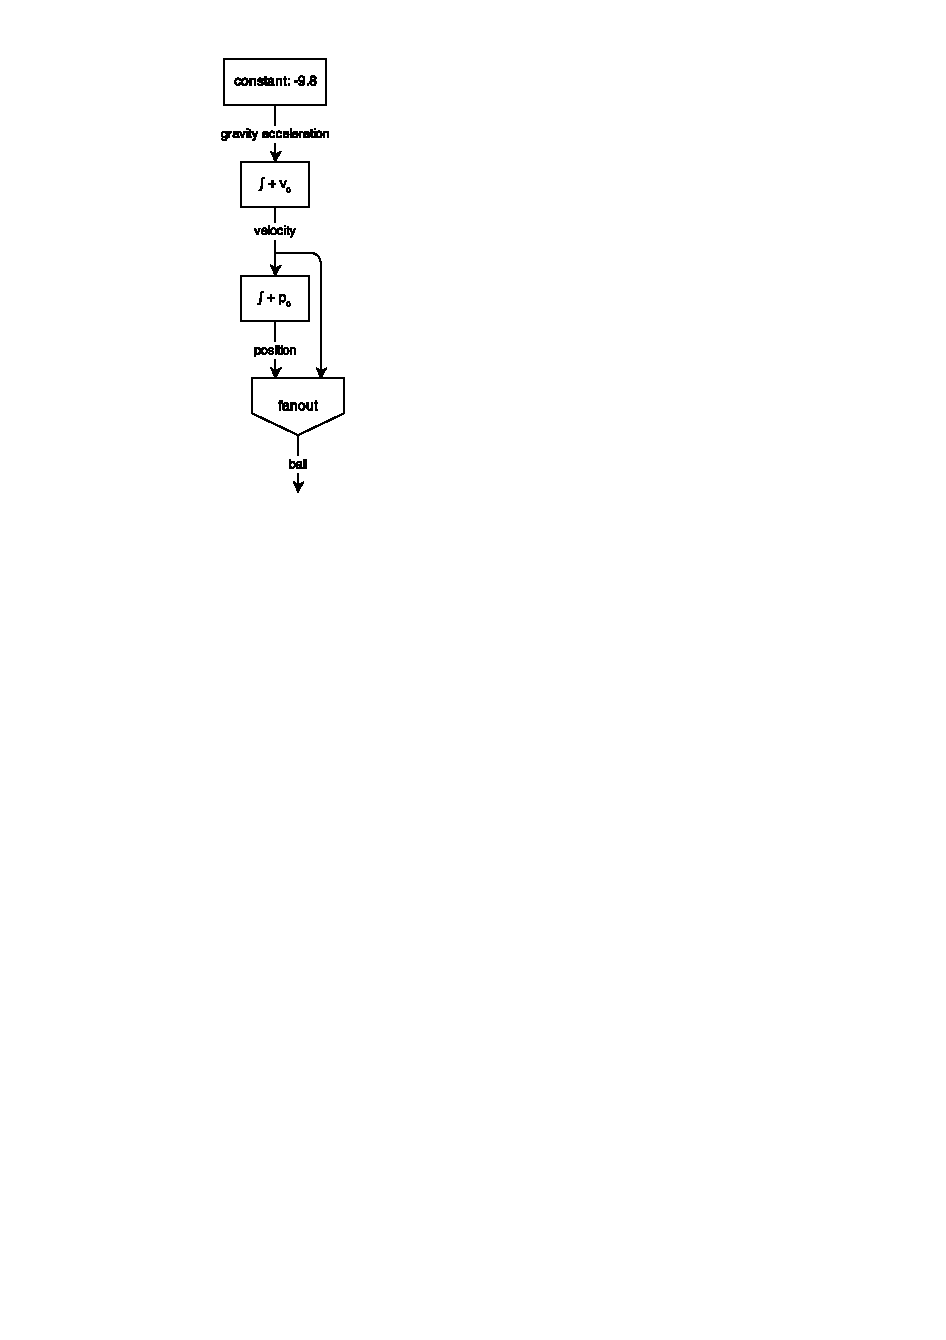
\includegraphics[width=0.2\linewidth,bb=0 0 65 215]{images/falling-ball.pdf}
    \caption{Flow diagram of a free falling ball}
    \label{fig:falling-ball}
\end{figure}

And then we call \texttt{rp.react} with a couple of other signal functions in
the processing pipeline: one of outputting, and the other to control when to
stop the simulation (after 3 seconds). We create a ``falling ball'' signal that
starts from height $10$ and velocity $0$ (initially stationary).

\begin{lstlisting}
rp.react(rp.compose(makeFallingBall(10.0, 0),
                    rp.lift(console.log),
                    rp.time(),
                    rp.lift(function (t) {
                              return t < 3;
                            })));
\end{lstlisting}

\texttt{rp.lift} ``lifts'' a pure function into a signal function \- this is
used for doing value processing and side effects (such as, in this example,
outputting and controlling when to stop).

\texttt{rp.time} constructs a constant signal function that will output the
current time (in seconds), it can be defined in terms of \texttt{constant}
and \texttt{integral} ($t = \int 1 \; dt$):

\begin{lstlisting}
function time () {
  return rp.compose(rp.constant(1), rp.integral());
}
\end{lstlisting}

Although signals are values that varies in time, we never manipulate this
underlying ``time'' directly, instead, if one needs to access the time one
should use the \texttt{rp.time} signal function. This is used in the example to
read the time and decide when to stop the simulation (when $t < 3$ condition
turns false).

When running the example, it produces an output like this:

\begin{verbatim}
{ vel: -0.9800000000000001, pos: 9.804 }
{ vel: -2.9400000000000004, pos: 9.412 }
{ vel: -4.9, pos: 8.824000000000002 }
{ vel: -6.860000000000001, pos: 8.040000000000001 }
{ vel: -8.820000000000002, pos: 7.0600000000000005 }
{ vel: -10.780000000000003, pos: 5.884 }
{ vel: -12.740000000000004, pos: 4.512 }
{ vel: -14.700000000000005, pos: 2.943999999999999 }
{ vel: -16.660000000000004, pos: 1.1799999999999986 }
{ vel: -18.620000000000005, pos: -0.780000000000002 }
{ vel: -20.580000000000005, pos: -2.9360000000000026 }
{ vel: -22.540000000000006, pos: -5.288000000000004 }
{ vel: -24.500000000000007, pos: -7.836000000000005 }
{ vel: -26.460000000000008, pos: -10.580000000000005 }
{ vel: -28.42000000000001, pos: -13.520000000000007 }
{ vel: -30.38000000000001, pos: -16.656000000000006 }
{ vel: -32.34000000000001, pos: -19.988000000000007 }
{ vel: -34.300000000000004, pos: -23.516000000000005 }
{ vel: -36.26, pos: -27.240000000000006 }
{ vel: -38.21999999999999, pos: -31.160000000000004 }
{ vel: -40.179999999999986, pos: -35.276 }
{ vel: -42.13999999999998, pos: -39.588 }
{ vel: -44.09999999999997, pos: -44.096 }
{ vel: -46.05999999999997, pos: -48.79999999999999 }
{ vel: -48.01999999999996, pos: -53.69999999999999 }
{ vel: -49.979999999999954, pos: -58.795999999999985 }
{ vel: -51.93999999999995, pos: -64.08799999999998 }
{ vel: -53.89999999999994, pos: -69.57599999999998 }
{ vel: -55.859999999999935, pos: -75.25999999999998 }
{ vel: -57.81999999999993, pos: -81.13999999999997 }
\end{verbatim}

\texttt{rp.react} uses the Euler method for solving Ordinary Differential
Equations (which is the signal function), and for that, it performs numerical
integrations using discrete values of time. Even though, in the code, we define
the equations in a continuous and intuitive manner.

Id desired, you can precisely control these time quantities as well as the
signal input value in the second (optional) parameter of \texttt{rp.react}. But
this tutorial will not cover this option.

The ball velocity increases linearly (modulo increases, but the direction is
negative), and it's position diminishes quadratically (if you plot the output
data you'll see clearly). Now let's model the collision with the floor.

For the collision, let's assume the floor is a plane at $y=0$. To model this
discontinuity in the ball's signal position and velocity we're going to use a
switch.

The function \texttt{rp.dSwitch} construct a signal function that has two
states: ``open'' and ``closed'' (switched). It starts open, but once closed it
remains that way forever. The difference between open and close is what signal
function the switch delegates it's working to.

By default it starts delegating it's working to the signal function passed as
the first parameter, once a test predicate is true (second parameter, a
function that maps a value to a boolean), then switch's third parameter is used
to construct another signal function that is then used following (and the switch
is in closed state).

Figure~\ref{fig:switch} represents graphical in a circuit-like diagram how is
the configuration of the switch. ``sf'' is the first parameter, the initial
signal function delegated by the switch; ``predicate'', the second parameter,
is the test that \- when passed \- will flip the switch to the newly generated
signal function ``sf\''', which is constructed by the switch's third parameter
``makeSF'', from the current signal's value.

\begin{figure}
    \centering
    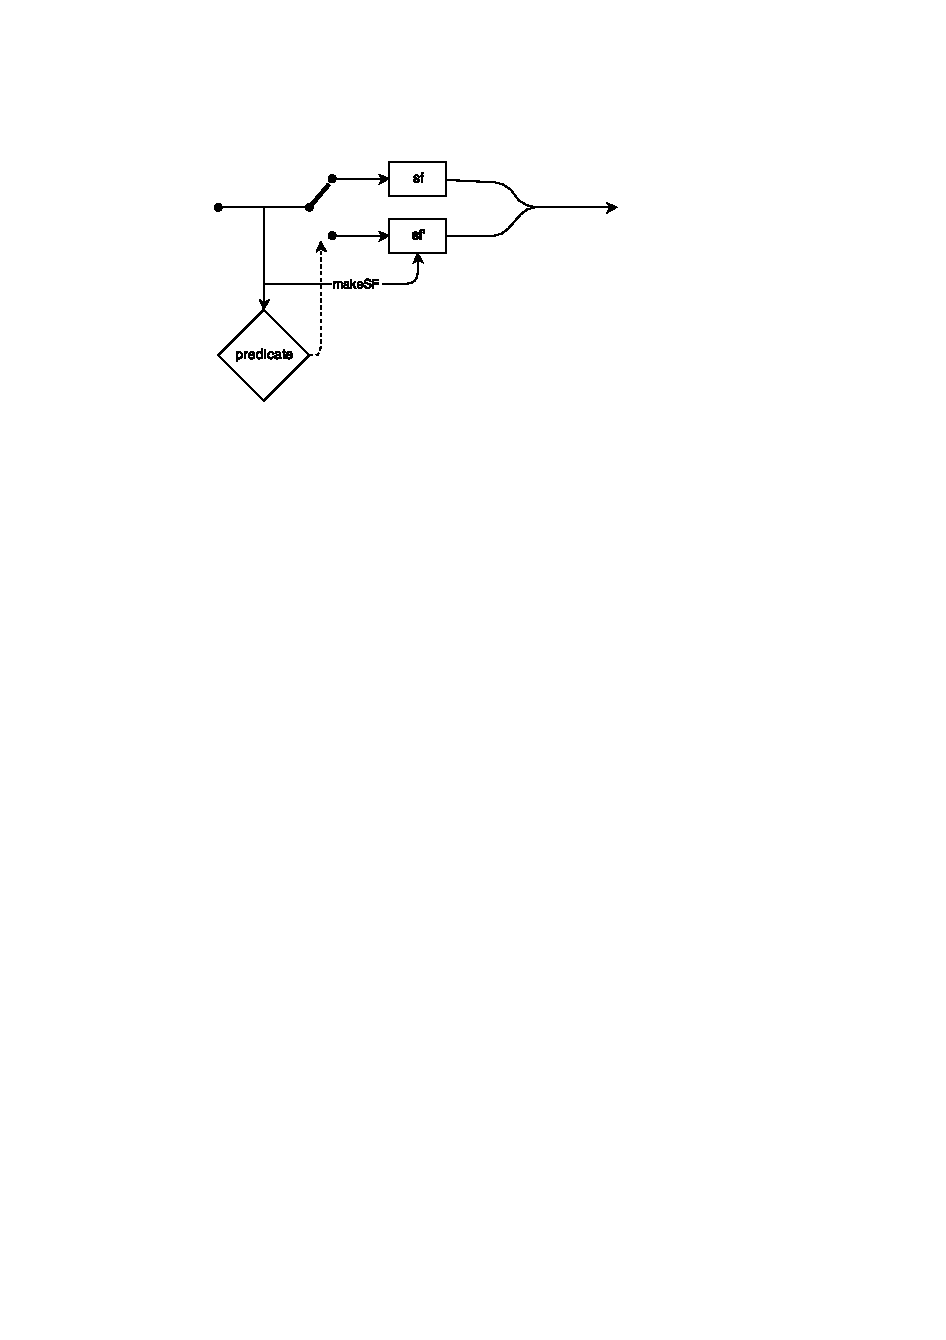
\includegraphics[width=\linewidth,bb=0 0 219 129]{images/rp-switch.pdf}
    \caption{Circuit diagram representation of a switch}
    \label{fig:switch}
\end{figure}

A switch in this case will model the position and velocity discontinuity that
happens when the ball collides with the ground. Our switch will have the
``falling ball'' as the first signal function, but when it's position is zero
(modeled by the predicate), the switch will change the signal to a ball that
starts from the ground but has it's velocity reflected (as to model a elastic
collision). The code is elegantly recursive:

\begin{lstlisting}
function bouncingBall(initialPos, initialVel) {
  var velocity    = rp.compose(rp.constant(-9.8),
                               rp.integral(initialVel)),
      position    = rp.compose(velocity,
                               rp.integral(initialPos)),
      fallingBall = rp.fanout(function (v, p) {
                                return {vel: v, pos: p};
                              },
                              velocity,
                              position);
  return rp.dSwitch(fallingBall,
                    function (ball) {
                      return ball.pos <= 0;
                    },
                    function (b) {
                       return bouncingBall(0, -.9 * b.vel);
                    });
}
\end{lstlisting}

A ``bouncing ball'' is a free falling ball that is switched by a ``bouncing
ball'' with the velocity reflected at 90\% of it's force (10\% is lost in the
not-perfectly elastic collision), when the position is zero.

To start, we construct it with initial position 10 and initial velocity zero.
Figure~\ref{fig:bouncing-ball} shows the plotting of the height and velocity of
the code above when simulated for 10 seconds. As can notice in the chart, the
height actually goes slightly below zero. That happens because of the time
quantization we discussed previously, and also that's why in the code we wrote
the predicate checking if the position is less or equal zero (instead of just
equal zero), because it may never be actually zero. Again, the quantization
value can be tweaked to be numerically as small as possible if one desires to
get a more precise simulation.

\begin{figure}
    \centering
    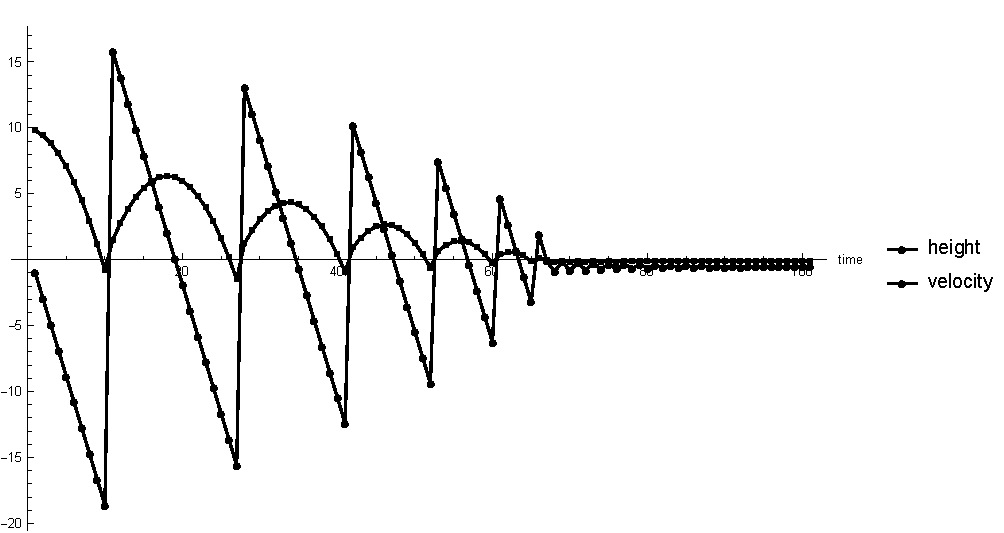
\includegraphics[width=\linewidth,bb=0 0 482 256]{images/bouncing-ball.pdf}
    \caption{Plot of height and velocity of a 10 second simulation of the falling ball}
    \label{fig:bouncing-ball}
\end{figure}

\subsection{Orbit}

Next we're going to build a system that requires a \textit{feedback loop}: a
Newtonian orbital system.

The system consists of a massive body which is orbited by a smaller body. To
simplify, we're considering that the massive body is stationary and it's not
affected by gravity - that of course is not physically correct, but if the mass
differences are big enough it's a feasible approximation. Also, we're going to
work with two dimensions, but one can see how easily this can be extended to
three dimensions.

Figure~\ref{fig:orbit} depicts the data flow of the system we're building. It's
very simple conceptually and also \- if implemented in the reactive programming
parading \- very simple in the code.

\begin{figure}
    \centering
    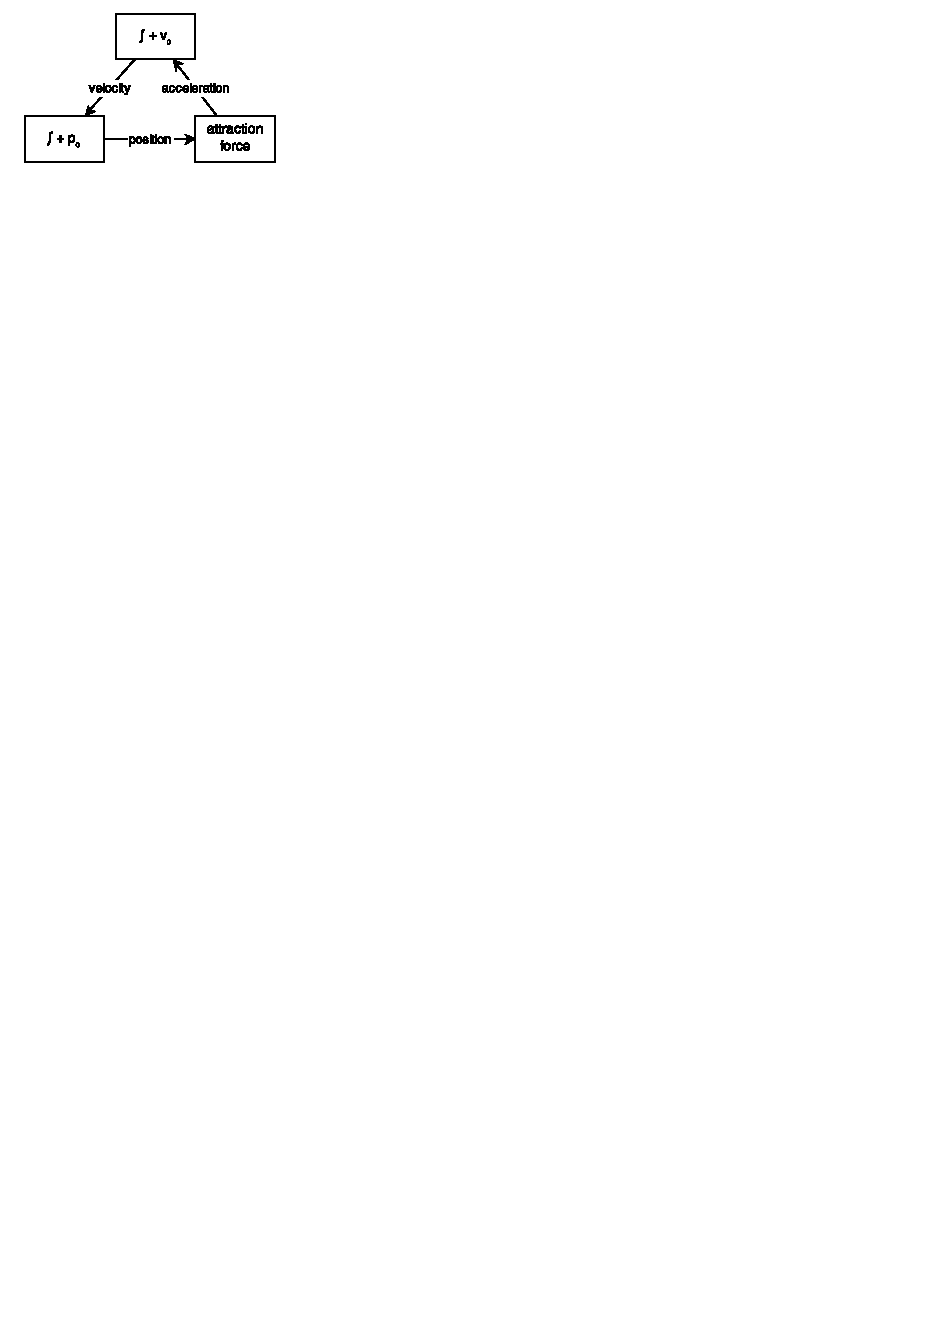
\includegraphics[width=0.8\linewidth,bb=0 0 133 82]{images/orbit.pdf}
    \caption{Flow diagram of the orbital feedback system}
    \label{fig:orbit}
\end{figure}

First, we start by defining the signal function that transform a position
signal into a gravity acceleration signal (the ``attraction force'' box in
Figure~\ref{fig:orbit}). This is a simplified implementation the ``universal
law of gravitation'':

\begin{equation}
    F = G \frac{m_1 m_2}{d^2}
\end{equation}
%
Where $G$ is the gravitational constant, $d$ is the distance between the two
bodies, $m_1$ and $m_2$ are the masses of the two bodies.

Our simplified version though, assumes $m_1 = m_2 = 1$, and the acceleration
can be calculated from the force and mass ($a = \frac{F}{m}$).

By a little of experimentation I arrived a value for $G$ of 100, in our
two-dimensional universe with unity masses, that value is able to create a
periodic orbit (without collapsing into a black-hole, neither spiraling out
into deep space). Following is the implementation of \texttt{force}, a simple
function that takes a position vector and returns an acceleration vector (we'll
see later how to lift that into a signal function):

\begin{lstlisting}
var G = 100; // nice gravitational constant

function force(p) {
  var d = Math.sqrt(Math.pow(p[0], 2) + Math.pow(p[1], 2));
  return [ G * -p[0] / Math.pow(d, 3),
           G * -p[1] / Math.pow(d, 3) ];
}
\end{lstlisting}

Next, is our complete system ``orbit'': the function takes the initial position
and initial velocity vectors and use the \texttt{rp.feedback} to build the
feedback loop:

\begin{lstlisting}
function orbit(initialPos, initialVel) {
  return rp.feedback(initialPos,
                     rp.compose(rp.lift(force),
                                rp.integral(initialVel),
                                rp.integral(initialPos)));
}
\end{lstlisting}

What \texttt{rp.feedback} does is taking it's first argument and feeding as a
``starting value'' to a signal function that is closed in itself (feeding from
it's own output signal from a infinitesimal time back). In this case, the
signal function we feedback is the body's position \- which is a dependency to
calculate itself.

Our \texttt{force} function is lifted into a signal function to calculate the
acceleration, then we integrate into the velocity, and integrate again into the
velocity. That output is fed back into the same processing. Please note that
\texttt{rp.integral} also works with vectors (Javascript arrays).

The limit of the \texttt{rp.feedback} of a signal function when time goes to
infinity, is the fixed point of that signal function.

To simulate the system this time, we also want the time value each step along
with the body's position. So we use \texttt{rp.fanout} to combine
\texttt{rp.time} and the orbit signal function into a function that console
logs that, and return just the time, which we pass through a stop condition
function (after 2000 seconds).

\begin{lstlisting}
rp.react(rp.compose(rp.fanout(function (t, p) {
                                console.log(t + ',' + p.join(','));
                                return t;
                              },
                              rp.time(),
                              orbit([60, 60], [1, -0.1])),
                    rp.lift(function (t) { return t < 2000; })));
\end{lstlisting}

Since the system does not run in real time, we don't have to wait for half an
hour for the simulation to complete a couple of orbits. The system runs pretty
fast, but if we wanted to make a real-time simulation, we could just place some
thread delays along the way.

Figure~\ref{fig:orbit-chart} shows the result of the simulation in a space-time
section (3D in this case).

\begin{figure}
    \centering
    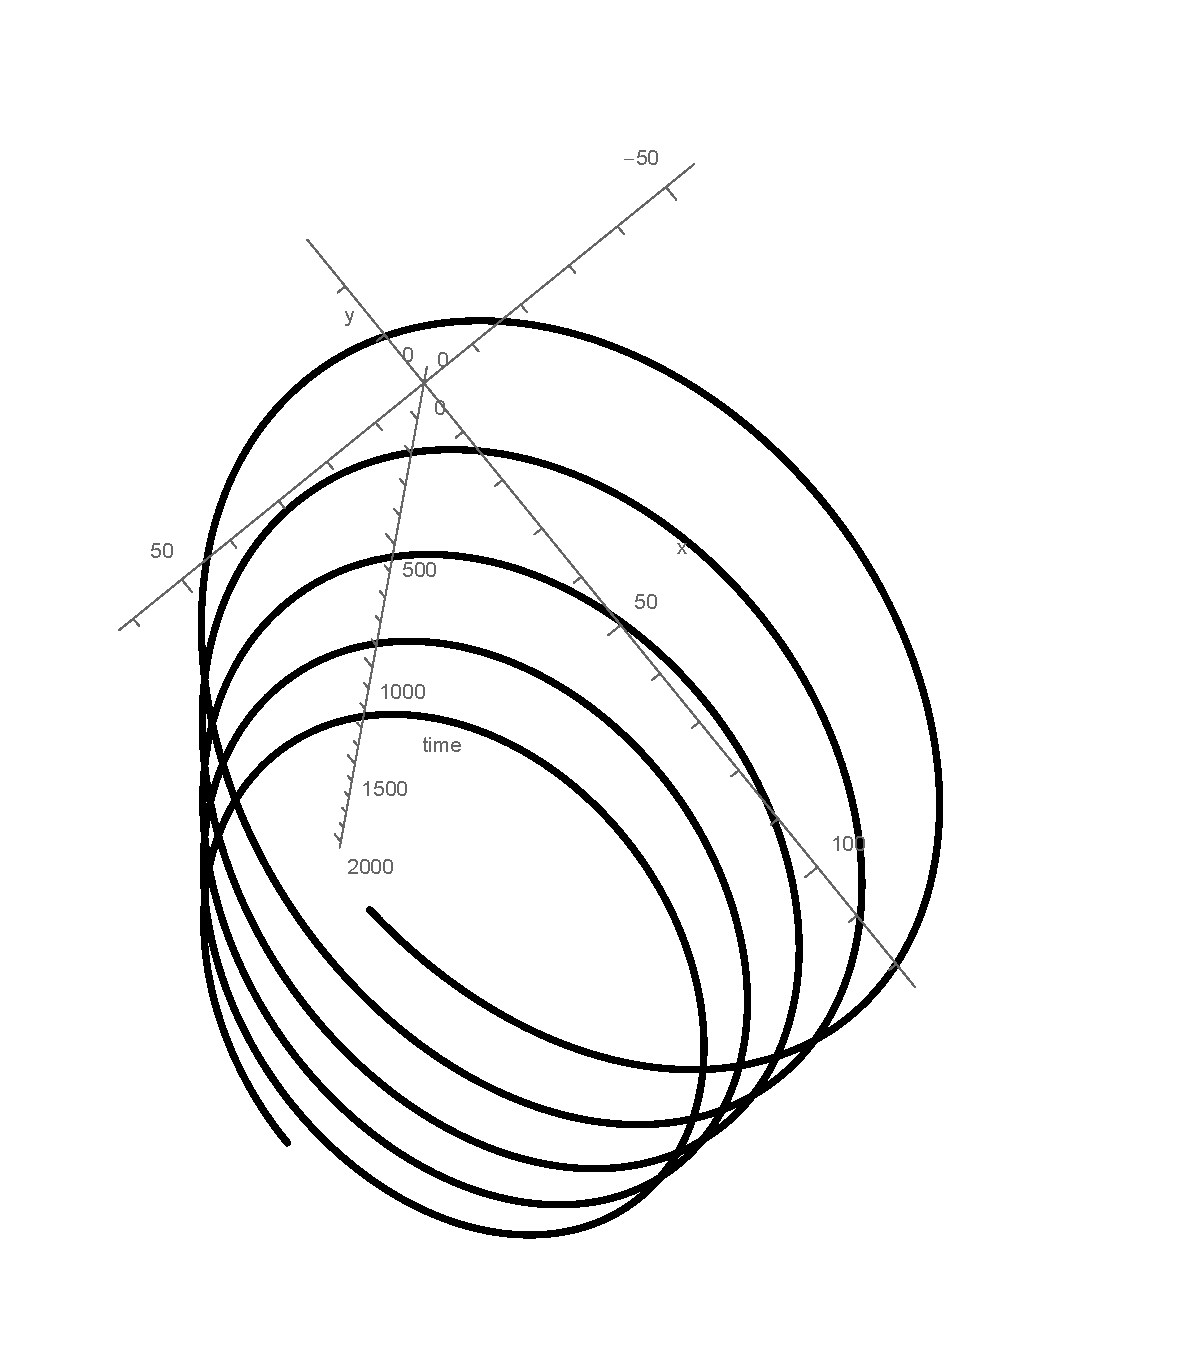
\includegraphics[width=\linewidth,bb=0 0 576 656]{images/orbit-chart.pdf}
    \caption{3D space-time section of the orbital system simulation in the 2D Newtonian universe}
    \label{fig:orbit-chart}
\end{figure}

\section{Conclusion}

We demonstrated two examples of reactive programming using Javascript, and I
hope it was clear to the reader the simplicity of specification of such systems
in comparison of how it would be like to program the same thing in the
canonical non-reactive paradigm.

Not only physical systems are a good fit for reactive programming, but also
other applications such as games, user interactive systems, text processing,
\textit{etc.}.

This tutorial was intended as a first reading, but There's a great deal of more
advanced material available in the Internet for who is further interested in
the subject.

\end{document}

